\section{Amazon}
\label{sec_amazon}

\IEEEPARstart{A}{mazon} hat um eine der größten online Verkaufsplattformen der Welt betreiben zu können eine stetig wachsende Infrastruktur geschaffen. Aus der dafür entwickelten Basis zur bedarfsgerechten Nutzung von Rechen- und Speicherressourcen sowie deren Management entstanden die Amazon Web Services. Mit Hilfe dieser Dienste ist es möglich Systemressourcen für die Entwicklung schnell abzurufen.

\subsection{Cloud und Amazon}
\label{sec_amazon_general}
Die Amazon Web Services stellen aufgrund der Vielfalt an Diensten, der Preisgestaltung sowie der Integration der Dienste untereinander als Marktführer im Bereich Cloud Computing. Die Produkte zum Management der Daten und Cloudinstanzen entstammen dabei der internen Nutzung Amazons, so z.B. die DynamoDB als Datenbank für große Datenmengen mit vorhersagbaren Zugriffszeiten, die ihren Ursprung in der Datenhaltung der Artikeldaten für den Amazon Onlinehandel hat oder EC2, der Dienst um virtuelle Server anzufordern, der zunächst in der internen Produktentwicklung für Amazon zum Einsatz kam. \cite{dynamo}

Um die entstandenen Dienste der Allgemeinheit zugänglich zu machen und so die vorhandene Infrastruktur besser ausnutzen zu können wurden die Dienste als Teil des public Cloud Angebots verfügbar gemacht.

\subsection{Service-Modelle}
\label{sec_amazon_delivery}
Die in Abbildung \ref{fig:amazon} dargestellten Dienste zeigen die Reichweite der angebotenen Services, dabei wird ersichtlich, dass neben den verschiedenen Zusatzdiensten der IaaS Bereich der Cloudanwendungen die größte Abdeckung bietet. Die IaaS sowie PaaS Angebote entstammen dabei vorwiegend dem Eigenbedarf an Lösungen und wurden mit fortschreitender Entwicklung für die public Cloud angepasst. Die Vertriebsplattform Amazon wird demnach auf Grundlage ebendieser Dienste betrieben. \cite{dynamo}

Die SaaS Lösungen des Unternehmens sind im Vergleich zu den übrigen Kategorien die jüngsten, wurde mit Amazon WorkMail erst 2015 der auf Unternehmen abzielende E-Maildienst von Amazon vorgestellt. \footnote{\url{http://www.crisp-research.com/amazon-workmail-amazon-aws-wachst-weiter-horizontal-im-cloud-stack/}}

\begin{figure*}
	\centering
	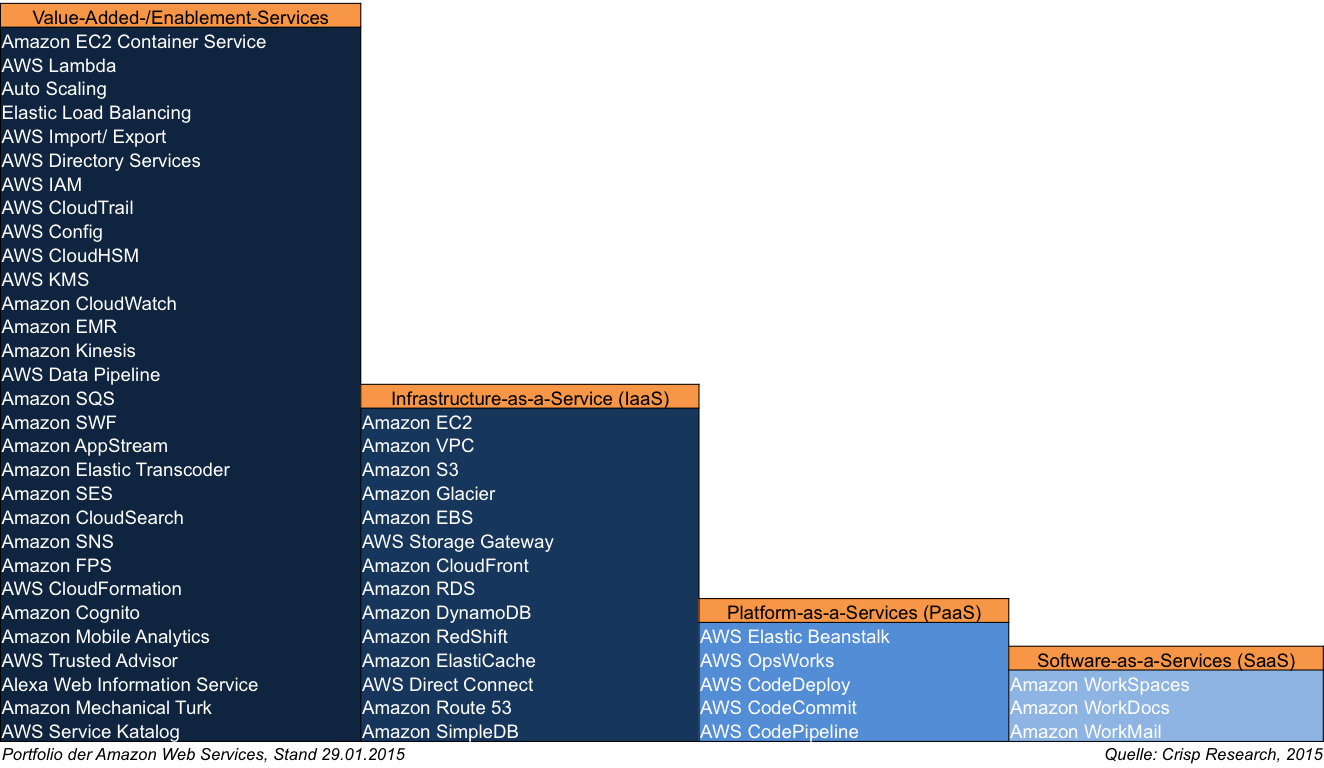
\includegraphics[width=0.8\linewidth]{images/Crisp-AWS-Portfolio_201501291}
	\caption{Amazon Web Services Portfolio }
	\label{fig:amazon}
\end{figure*}

\subsection{Betriebsmodelle}
\label{sec_amazon_deployment}
Die unterschiedlichen Cloud Dienste werden von Amazon als Teil ihres public Cloud Angebots betrieben und in der Regel als Shared Public Cloud angeboten.

Amazon bietet jedoch auch die Möglichkeit eine Dedicated Public Cloud zu betreiben, dieses wird als "Amazon Virtual Private Cloud (Amazon VPC)"\footnote{url{http://aws.amazon.com/de/vpc/}} bezeichnet. Dabei gilt es allerdings zu beachten, dass es sich nur um virtuell private Server handelt, was es zwar erlaubt virtuelle Netzwerke von selbst konfigurierten  Systemen erstellen zu können, diese jedoch die darunterliegende Hardware mit anderen Anwendungen teilen. 

Eine Möglichkeit eine Private Appliance, Self Hosted Private oder Hosted Private Cloud mit den Mitteln der Amazon Web Services zu betreiben gibt es nicht. \cite{amazonPrivate}
